% Options for packages loaded elsewhere
\PassOptionsToPackage{unicode}{hyperref}
\PassOptionsToPackage{hyphens}{url}
\documentclass[
  12pt,
]{article}
\usepackage{xcolor}
\usepackage[margin=1in]{geometry}
\usepackage{amsmath,amssymb}
\setcounter{secnumdepth}{-\maxdimen} % remove section numbering
\usepackage{iftex}
\ifPDFTeX
  \usepackage[T1]{fontenc}
  \usepackage[utf8]{inputenc}
  \usepackage{textcomp} % provide euro and other symbols
\else % if luatex or xetex
  \usepackage{unicode-math} % this also loads fontspec
  \defaultfontfeatures{Scale=MatchLowercase}
  \defaultfontfeatures[\rmfamily]{Ligatures=TeX,Scale=1}
\fi
\usepackage{lmodern}
\ifPDFTeX\else
  % xetex/luatex font selection
  \setmainfont[]{Noto Sans CJK TC}
\fi
% Use upquote if available, for straight quotes in verbatim environments
\IfFileExists{upquote.sty}{\usepackage{upquote}}{}
\IfFileExists{microtype.sty}{% use microtype if available
  \usepackage[]{microtype}
  \UseMicrotypeSet[protrusion]{basicmath} % disable protrusion for tt fonts
}{}
\makeatletter
\@ifundefined{KOMAClassName}{% if non-KOMA class
  \IfFileExists{parskip.sty}{%
    \usepackage{parskip}
  }{% else
    \setlength{\parindent}{0pt}
    \setlength{\parskip}{6pt plus 2pt minus 1pt}}
}{% if KOMA class
  \KOMAoptions{parskip=half}}
\makeatother
\usepackage{color}
\usepackage{fancyvrb}
\newcommand{\VerbBar}{|}
\newcommand{\VERB}{\Verb[commandchars=\\\{\}]}
\DefineVerbatimEnvironment{Highlighting}{Verbatim}{commandchars=\\\{\}}
% Add ',fontsize=\small' for more characters per line
\usepackage{framed}
\definecolor{shadecolor}{RGB}{248,248,248}
\newenvironment{Shaded}{\begin{snugshade}}{\end{snugshade}}
\newcommand{\AlertTok}[1]{\textcolor[rgb]{0.94,0.16,0.16}{#1}}
\newcommand{\AnnotationTok}[1]{\textcolor[rgb]{0.56,0.35,0.01}{\textbf{\textit{#1}}}}
\newcommand{\AttributeTok}[1]{\textcolor[rgb]{0.13,0.29,0.53}{#1}}
\newcommand{\BaseNTok}[1]{\textcolor[rgb]{0.00,0.00,0.81}{#1}}
\newcommand{\BuiltInTok}[1]{#1}
\newcommand{\CharTok}[1]{\textcolor[rgb]{0.31,0.60,0.02}{#1}}
\newcommand{\CommentTok}[1]{\textcolor[rgb]{0.56,0.35,0.01}{\textit{#1}}}
\newcommand{\CommentVarTok}[1]{\textcolor[rgb]{0.56,0.35,0.01}{\textbf{\textit{#1}}}}
\newcommand{\ConstantTok}[1]{\textcolor[rgb]{0.56,0.35,0.01}{#1}}
\newcommand{\ControlFlowTok}[1]{\textcolor[rgb]{0.13,0.29,0.53}{\textbf{#1}}}
\newcommand{\DataTypeTok}[1]{\textcolor[rgb]{0.13,0.29,0.53}{#1}}
\newcommand{\DecValTok}[1]{\textcolor[rgb]{0.00,0.00,0.81}{#1}}
\newcommand{\DocumentationTok}[1]{\textcolor[rgb]{0.56,0.35,0.01}{\textbf{\textit{#1}}}}
\newcommand{\ErrorTok}[1]{\textcolor[rgb]{0.64,0.00,0.00}{\textbf{#1}}}
\newcommand{\ExtensionTok}[1]{#1}
\newcommand{\FloatTok}[1]{\textcolor[rgb]{0.00,0.00,0.81}{#1}}
\newcommand{\FunctionTok}[1]{\textcolor[rgb]{0.13,0.29,0.53}{\textbf{#1}}}
\newcommand{\ImportTok}[1]{#1}
\newcommand{\InformationTok}[1]{\textcolor[rgb]{0.56,0.35,0.01}{\textbf{\textit{#1}}}}
\newcommand{\KeywordTok}[1]{\textcolor[rgb]{0.13,0.29,0.53}{\textbf{#1}}}
\newcommand{\NormalTok}[1]{#1}
\newcommand{\OperatorTok}[1]{\textcolor[rgb]{0.81,0.36,0.00}{\textbf{#1}}}
\newcommand{\OtherTok}[1]{\textcolor[rgb]{0.56,0.35,0.01}{#1}}
\newcommand{\PreprocessorTok}[1]{\textcolor[rgb]{0.56,0.35,0.01}{\textit{#1}}}
\newcommand{\RegionMarkerTok}[1]{#1}
\newcommand{\SpecialCharTok}[1]{\textcolor[rgb]{0.81,0.36,0.00}{\textbf{#1}}}
\newcommand{\SpecialStringTok}[1]{\textcolor[rgb]{0.31,0.60,0.02}{#1}}
\newcommand{\StringTok}[1]{\textcolor[rgb]{0.31,0.60,0.02}{#1}}
\newcommand{\VariableTok}[1]{\textcolor[rgb]{0.00,0.00,0.00}{#1}}
\newcommand{\VerbatimStringTok}[1]{\textcolor[rgb]{0.31,0.60,0.02}{#1}}
\newcommand{\WarningTok}[1]{\textcolor[rgb]{0.56,0.35,0.01}{\textbf{\textit{#1}}}}
\usepackage{graphicx}
\makeatletter
\newsavebox\pandoc@box
\newcommand*\pandocbounded[1]{% scales image to fit in text height/width
  \sbox\pandoc@box{#1}%
  \Gscale@div\@tempa{\textheight}{\dimexpr\ht\pandoc@box+\dp\pandoc@box\relax}%
  \Gscale@div\@tempb{\linewidth}{\wd\pandoc@box}%
  \ifdim\@tempb\p@<\@tempa\p@\let\@tempa\@tempb\fi% select the smaller of both
  \ifdim\@tempa\p@<\p@\scalebox{\@tempa}{\usebox\pandoc@box}%
  \else\usebox{\pandoc@box}%
  \fi%
}
% Set default figure placement to htbp
\def\fps@figure{htbp}
\makeatother
\setlength{\emergencystretch}{3em} % prevent overfull lines
\providecommand{\tightlist}{%
  \setlength{\itemsep}{0pt}\setlength{\parskip}{0pt}}
\usepackage{booktabs}
\usepackage{longtable}
\usepackage{array}
\usepackage{multirow}
\usepackage{wrapfig}
\usepackage{float}
\usepackage{colortbl}
\usepackage{pdflscape}
\usepackage{tabu}
\usepackage{threeparttable}
\usepackage{threeparttablex}
\usepackage[normalem]{ulem}
\usepackage{makecell}
\usepackage{xcolor}
\usepackage{bookmark}
\IfFileExists{xurl.sty}{\usepackage{xurl}}{} % add URL line breaks if available
\urlstyle{same}
\hypersetup{
  pdftitle={work\_2 作業報告},
  hidelinks,
  pdfcreator={LaTeX via pandoc}}

\title{work\_2 作業報告}
\author{}
\date{\vspace{-2.5em}2025-09-30}

\begin{document}
\maketitle

{
\setcounter{tocdepth}{2}
\tableofcontents
}
\subsection{安裝工具來做描述性統計}\label{ux5b89ux88ddux5de5ux5177ux4f86ux505aux63cfux8ff0ux6027ux7d71ux8a08}

\begin{Shaded}
\begin{Highlighting}[]
\FunctionTok{install.packages}\NormalTok{(}\FunctionTok{c}\NormalTok{(}\StringTok{"psych"}\NormalTok{, }\StringTok{"emmeans"}\NormalTok{))}
\FunctionTok{install.packages}\NormalTok{(}\StringTok{"emmeans"}\NormalTok{)}
\end{Highlighting}
\end{Shaded}

\subsection{載入套件}\label{ux8f09ux5165ux5957ux4ef6}

\begin{Shaded}
\begin{Highlighting}[]
\FunctionTok{library}\NormalTok{(psych)}
\FunctionTok{library}\NormalTok{(emmeans)}
\end{Highlighting}
\end{Shaded}

\begin{verbatim}
## Welcome to emmeans.
## Caution: You lose important information if you filter this package's results.
## See '? untidy'
\end{verbatim}

\begin{Shaded}
\begin{Highlighting}[]
\FunctionTok{library}\NormalTok{(dplyr)}
\end{Highlighting}
\end{Shaded}

\begin{verbatim}
## 
## Attaching package: 'dplyr'
\end{verbatim}

\begin{verbatim}
## The following objects are masked from 'package:stats':
## 
##     filter, lag
\end{verbatim}

\begin{verbatim}
## The following objects are masked from 'package:base':
## 
##     intersect, setdiff, setequal, union
\end{verbatim}

\begin{Shaded}
\begin{Highlighting}[]
\FunctionTok{library}\NormalTok{(knitr)}
\FunctionTok{library}\NormalTok{(kableExtra)}
\end{Highlighting}
\end{Shaded}

\begin{verbatim}
## 
## Attaching package: 'kableExtra'
\end{verbatim}

\begin{verbatim}
## The following object is masked from 'package:dplyr':
## 
##     group_rows
\end{verbatim}

\begin{Shaded}
\begin{Highlighting}[]
\FunctionTok{library}\NormalTok{(tidyr)}
\FunctionTok{library}\NormalTok{(ggplot2)}
\end{Highlighting}
\end{Shaded}

\begin{verbatim}
## 
## Attaching package: 'ggplot2'
\end{verbatim}

\begin{verbatim}
## The following objects are masked from 'package:psych':
## 
##     %+%, alpha
\end{verbatim}

\section{0. 輸入CSV}\label{ux8f38ux5165csv}

\begin{Shaded}
\begin{Highlighting}[]
\NormalTok{emg\_df }\OtherTok{\textless{}{-}} \FunctionTok{data.frame}\NormalTok{(}
  \AttributeTok{Sex    =} \FunctionTok{c}\NormalTok{(}\StringTok{"M"}\NormalTok{,}\StringTok{"M"}\NormalTok{,}\StringTok{"F"}\NormalTok{,}\StringTok{"M"}\NormalTok{,}\StringTok{"M"}\NormalTok{,}\StringTok{"M"}\NormalTok{,}\StringTok{"F"}\NormalTok{,}\StringTok{"M"}\NormalTok{,}\StringTok{"F"}\NormalTok{,}\StringTok{"F"}\NormalTok{),}
  \AttributeTok{Hand   =} \FunctionTok{rep}\NormalTok{(}\StringTok{"Right"}\NormalTok{, }\DecValTok{10}\NormalTok{),}
  \AttributeTok{Muscle =} \FunctionTok{rep}\NormalTok{(}\StringTok{"forearm"}\NormalTok{, }\DecValTok{10}\NormalTok{),}
  \AttributeTok{basic  =} \FunctionTok{c}\NormalTok{(}\FloatTok{0.116}\NormalTok{,}\FloatTok{0.133}\NormalTok{,}\FloatTok{0.085}\NormalTok{,}\FloatTok{0.140}\NormalTok{,}\FloatTok{0.134}\NormalTok{,}\FloatTok{0.204}\NormalTok{,}\FloatTok{0.128}\NormalTok{,}\FloatTok{0.137}\NormalTok{,}\FloatTok{0.142}\NormalTok{,}\FloatTok{0.137}\NormalTok{),}
  \AttributeTok{grip   =} \FunctionTok{c}\NormalTok{(}\FloatTok{0.769}\NormalTok{,}\FloatTok{0.521}\NormalTok{,}\FloatTok{0.749}\NormalTok{,}\FloatTok{0.708}\NormalTok{,}\FloatTok{0.652}\NormalTok{,}\FloatTok{1.10}\NormalTok{,}\FloatTok{0.785}\NormalTok{,}\FloatTok{0.820}\NormalTok{,}\FloatTok{0.634}\NormalTok{,}\FloatTok{0.729}\NormalTok{)}
\NormalTok{)}
\end{Highlighting}
\end{Shaded}

\section{第一題:輸出CSV}\label{ux7b2cux4e00ux984cux8f38ux51facsv}

\begin{Shaded}
\begin{Highlighting}[]
\FunctionTok{write.csv}\NormalTok{(emg\_df, }\StringTok{"emg\_data.csv"}\NormalTok{)}
\end{Highlighting}
\end{Shaded}

\begin{quote}
先製作 long data 方便後續分析
\end{quote}

\begin{Shaded}
\begin{Highlighting}[]
\NormalTok{dat\_long }\OtherTok{\textless{}{-}}\NormalTok{ emg\_df }\SpecialCharTok{\%\textgreater{}\%}
  \FunctionTok{mutate}\NormalTok{(}\AttributeTok{ID =} \FunctionTok{paste0}\NormalTok{(}\StringTok{"ST\_"}\NormalTok{, }\FunctionTok{row\_number}\NormalTok{())) }\SpecialCharTok{\%\textgreater{}\%}
  \FunctionTok{pivot\_longer}\NormalTok{(}
    \AttributeTok{cols      =} \FunctionTok{c}\NormalTok{(basic, grip),}
    \AttributeTok{names\_to  =} \StringTok{"action"}\NormalTok{,}
    \AttributeTok{values\_to =} \StringTok{"EEG"}
\NormalTok{  )}
\end{Highlighting}
\end{Shaded}

\section{第二題:繪製 ``action 因子''之描述統計、繪製 ``sex
性別因子''之描述統計}\label{ux7b2cux4e8cux984cux7e6aux88fd-action-ux56e0ux5b50ux4e4bux63cfux8ff0ux7d71ux8a08ux7e6aux88fd-sex-ux6027ux5225ux56e0ux5b50ux4e4bux63cfux8ff0ux7d71ux8a08}

\begin{Shaded}
\begin{Highlighting}[]
\NormalTok{desc\_action }\OtherTok{\textless{}{-}}\NormalTok{ psych}\SpecialCharTok{::}\FunctionTok{describeBy}\NormalTok{(dat\_long}\SpecialCharTok{$}\NormalTok{EEG, }\AttributeTok{group =}\NormalTok{ dat\_long}\SpecialCharTok{$}\NormalTok{action, }\AttributeTok{mat =} \ConstantTok{TRUE}\NormalTok{) }\SpecialCharTok{\%\textgreater{}\%}
  \FunctionTok{select}\NormalTok{(}\AttributeTok{group =}\NormalTok{ group1, }\AttributeTok{N =}\NormalTok{ n, }\AttributeTok{Mean =}\NormalTok{ mean, }\AttributeTok{SD =}\NormalTok{ sd, }\AttributeTok{Median =}\NormalTok{ median, }\AttributeTok{Min =}\NormalTok{ min, }\AttributeTok{Max =}\NormalTok{ max, }\AttributeTok{Skew =}\NormalTok{ skew, }\AttributeTok{Kurtosis =}\NormalTok{ kurtosis, }\AttributeTok{SEM =}\NormalTok{ se) }

\NormalTok{desc\_action }\SpecialCharTok{\%\textgreater{}\%}
  \FunctionTok{kable}\NormalTok{(}\AttributeTok{align =} \StringTok{"l"}\NormalTok{, }\AttributeTok{digits =} \DecValTok{2}\NormalTok{, }\AttributeTok{row.names =} \ConstantTok{FALSE}\NormalTok{,}
        \AttributeTok{caption =} \StringTok{"Descriptive Statistics by Action"}\NormalTok{) }\SpecialCharTok{\%\textgreater{}\%}
  \FunctionTok{kable\_styling}\NormalTok{(}\AttributeTok{bootstrap\_options =} \FunctionTok{c}\NormalTok{(}\StringTok{"bordered"}\NormalTok{, }\StringTok{"responsive"}\NormalTok{, }\StringTok{"striped"}\NormalTok{), }\AttributeTok{full\_width =} \ConstantTok{FALSE}\NormalTok{)}
\end{Highlighting}
\end{Shaded}

\begin{longtable}[t]{llllllllll}
\caption{\label{tab:describe}Descriptive Statistics by Action}\\
\toprule
group & N & Mean & SD & Median & Min & Max & Skew & Kurtosis & SEM\\
\midrule
basic & 10 & 0.14 & 0.03 & 0.14 & 0.09 & 0.2 & 0.72 & 0.85 & 0.01\\
grip & 10 & 0.75 & 0.15 & 0.74 & 0.52 & 1.1 & 0.88 & 0.50 & 0.05\\
\bottomrule
\end{longtable}

\begin{quote}
在 靜止 (basic) 條件下,前臂肌群肌電活動相對較低,平均值為 0.136 (SD =
0.029, SE = 0.009),數值範圍介於 0.085 至 0.204
之間。資料分布近似常態,呈現輕度右偏 (偏態 = 0.72),峰度為
0.85,顯示受試者間數值相當集中且穩定。

在 抓握 (grip) 條件下,前臂肌群肌電活動顯著增加,平均值為 0.747 (SD =
0.151, SE = 0.048),數值範圍介於 0.521 至 1.100
之間。分布同樣近似常態,但右偏程度較高 (偏態 = 0.88),峰度較低
(0.50),顯示不同受試者在肌肉收縮時的變異性較大。

整體而言,抓握動作下的肌電活動約為靜止狀態的 5.5
倍,且受試者間差異更為明顯。
\end{quote}

\begin{Shaded}
\begin{Highlighting}[]
\NormalTok{desc\_basic }\OtherTok{\textless{}{-}}\NormalTok{ psych}\SpecialCharTok{::}\FunctionTok{describeBy}\NormalTok{(emg\_df}\SpecialCharTok{$}\NormalTok{basic, }\AttributeTok{group =}\NormalTok{ emg\_df}\SpecialCharTok{$}\NormalTok{Sex, }\AttributeTok{mat =} \ConstantTok{TRUE}\NormalTok{) }\SpecialCharTok{\%\textgreater{}\%}
  \FunctionTok{select}\NormalTok{(}\AttributeTok{group =}\NormalTok{ group1, }\AttributeTok{N =}\NormalTok{ n, }\AttributeTok{Mean =}\NormalTok{ mean, }\AttributeTok{SD =}\NormalTok{ sd, }\AttributeTok{Median =}\NormalTok{ median, }\AttributeTok{Min =}\NormalTok{ min, }\AttributeTok{Max =}\NormalTok{ max, }\AttributeTok{Skew =}\NormalTok{ skew, }\AttributeTok{Kurtosis =}\NormalTok{ kurtosis, }\AttributeTok{SEM =}\NormalTok{ se) }\SpecialCharTok{\%\textgreater{}\%}
  \FunctionTok{mutate}\NormalTok{(}\AttributeTok{Action =} \StringTok{"basic"}\NormalTok{)}

\NormalTok{desc\_grip }\OtherTok{\textless{}{-}}\NormalTok{ psych}\SpecialCharTok{::}\FunctionTok{describeBy}\NormalTok{(emg\_df}\SpecialCharTok{$}\NormalTok{grip, }\AttributeTok{group =}\NormalTok{ emg\_df}\SpecialCharTok{$}\NormalTok{Sex, }\AttributeTok{mat =} \ConstantTok{TRUE}\NormalTok{) }\SpecialCharTok{\%\textgreater{}\%}
  \FunctionTok{select}\NormalTok{(}\AttributeTok{group =}\NormalTok{ group1, }\AttributeTok{N =}\NormalTok{ n, }\AttributeTok{Mean =}\NormalTok{ mean, }\AttributeTok{SD =}\NormalTok{ sd, }\AttributeTok{Median =}\NormalTok{ median, }\AttributeTok{Min =}\NormalTok{ min, }\AttributeTok{Max =}\NormalTok{ max, }\AttributeTok{Skew =}\NormalTok{ skew, }\AttributeTok{Kurtosis =}\NormalTok{ kurtosis, }\AttributeTok{SEM =}\NormalTok{ se) }\SpecialCharTok{\%\textgreater{}\%}
  \FunctionTok{mutate}\NormalTok{(}\AttributeTok{Action =} \StringTok{"grip"}\NormalTok{)}

\NormalTok{desc\_table }\OtherTok{\textless{}{-}} \FunctionTok{bind\_rows}\NormalTok{(desc\_basic, desc\_grip)}

\NormalTok{desc\_table }\SpecialCharTok{\%\textgreater{}\%}
  \FunctionTok{kable}\NormalTok{(}\AttributeTok{align =} \StringTok{"l"}\NormalTok{, }\AttributeTok{digits =} \DecValTok{2}\NormalTok{, }\AttributeTok{row.names =} \ConstantTok{FALSE}\NormalTok{,}
        \AttributeTok{caption =} \StringTok{"Descriptive Statistics by Sex and Action"}\NormalTok{) }\SpecialCharTok{\%\textgreater{}\%}
  \FunctionTok{kable\_styling}\NormalTok{(}\AttributeTok{bootstrap\_options =} \FunctionTok{c}\NormalTok{(}\StringTok{"bordered"}\NormalTok{, }\StringTok{"responsive"}\NormalTok{, }\StringTok{"striped"}\NormalTok{), }\AttributeTok{full\_width =} \ConstantTok{FALSE}\NormalTok{)}
\end{Highlighting}
\end{Shaded}

\begin{longtable}[t]{lllllllllll}
\caption{\label{tab:describeBy-sex-table}Descriptive Statistics by Sex and Action}\\
\toprule
group & N & Mean & SD & Median & Min & Max & Skew & Kurtosis & SEM & Action\\
\midrule
F & 4 & 0.12 & 0.03 & 0.13 & 0.09 & 0.14 & -0.64 & -1.76 & 0.01 & basic\\
M & 6 & 0.14 & 0.03 & 0.14 & 0.12 & 0.20 & 1.12 & -0.40 & 0.01 & basic\\
F & 4 & 0.72 & 0.06 & 0.74 & 0.63 & 0.78 & -0.46 & -1.84 & 0.03 & grip\\
M & 6 & 0.76 & 0.20 & 0.74 & 0.52 & 1.10 & 0.53 & -1.10 & 0.08 & grip\\
\bottomrule
\end{longtable}

\begin{quote}
在靜止條件下,男性的肌電活動平均略高於女性,且分布較分散;在抓握條件下,男女平均值相近,但男性的變異度顯著較大。
\end{quote}

\section{第三題:請寫出本實驗的實驗設計(
包含因子(獨立變數)、水準、受測者間/受測者內、相依變數(含單位)等)}\label{ux7b2cux4e09ux984cux8acbux5bebux51faux672cux5be6ux9a57ux7684ux5be6ux9a57ux8a2dux8a08-ux5305ux542bux56e0ux5b50ux7368ux7acbux8b8aux6578ux6c34ux6e96ux53d7ux6e2cux8005ux9593ux53d7ux6e2cux8005ux5167ux76f8ux4f9dux8b8aux6578ux542bux55aeux4f4dux7b49}

\begin{itemize}
\item
  設計:二因子重複量測設計(repeated measures design)

  \begin{enumerate}
  \def\labelenumi{\arabic{enumi}.}
  \item
    受試者間因子(Between-subjects):Sex(2 水準:Male、Female)
  \item
    受試者內因子(Within-subjects):action(2
    水準:basic=靜止、grip=抓握)
  \end{enumerate}
\item
  相依變數(Dependent Variable):前臂肌群 EMG 電位,已對個人 MVC
  正規化後的百分比,單位 \%MVC。
\item
  樣本:10 位健康成人(6 男、4 女),每位皆完成 2 種動作的量測。
\item
  目的:檢驗動作(靜止 vs 抓握)與性別(男 vs 女)對 \%MVC
  之主效應與交互作用。
\end{itemize}

\section{第四題:進行 ANOVA 分析(請貼 R
執行結果圖),並寫出主效果及交互作用項之顯著性(僅需寫出達顯著水準者)。}\label{ux7b2cux56dbux984cux9032ux884c-anova-ux5206ux6790ux8acbux8cbc-r-ux57f7ux884cux7d50ux679cux5716ux4e26ux5bebux51faux4e3bux6548ux679cux53caux4ea4ux4e92ux4f5cux7528ux9805ux4e4bux986fux8457ux6027ux50c5ux9700ux5bebux51faux9054ux986fux8457ux6c34ux6e96ux8005}

\begin{Shaded}
\begin{Highlighting}[]
\NormalTok{TwoBetweenData.aov }\OtherTok{\textless{}{-}} \FunctionTok{aov}\NormalTok{(EEG }\SpecialCharTok{\textasciitilde{}}\NormalTok{ Sex }\SpecialCharTok{*}\NormalTok{ action, }\AttributeTok{data =}\NormalTok{ dat\_long)}
\FunctionTok{summary}\NormalTok{(TwoBetweenData.aov)}
\end{Highlighting}
\end{Shaded}

\begin{verbatim}
##             Df Sum Sq Mean Sq F value   Pr(>F)    
## Sex          1 0.0041  0.0041   0.312    0.584    
## action       1 1.8672  1.8672 142.318 2.24e-09 ***
## Sex:action   1 0.0003  0.0003   0.025    0.877    
## Residuals   16 0.2099  0.0131                     
## ---
## Signif. codes:  0 '***' 0.001 '**' 0.01 '*' 0.05 '.' 0.1 ' ' 1
\end{verbatim}

\begin{quote}
ANOVA 結果顯示,\textbf{動作的主效果達顯著} {[}F(1,16)=142.32,
p\textless.001{]},表示不同動作 (basic vs.~grip) 在 EEG
上有顯著差異。\textbf{性別主效果不顯著} {[}F(1,16)=0.31,
p=.584{]},\textbf{性別與動作的交互作用亦不顯著} {[}F(1,16)=0.03,
p=.877{]}。
\end{quote}

\section{第五題:請以``bon''方法進行主效果(``sex
性別'')事後檢定完成分群並說明其意義}\label{ux7b2cux4e94ux984cux8acbux4ee5bonux65b9ux6cd5ux9032ux884cux4e3bux6548ux679csex-ux6027ux5225ux4e8bux5f8cux6aa2ux5b9aux5b8cux6210ux5206ux7fa4ux4e26ux8aaaux660eux5176ux610fux7fa9}

\begin{Shaded}
\begin{Highlighting}[]
\NormalTok{TwoBetweenData.aov }\OtherTok{\textless{}{-}} \FunctionTok{aov}\NormalTok{(EEG }\SpecialCharTok{\textasciitilde{}}\NormalTok{ Sex }\SpecialCharTok{*}\NormalTok{ action, }\AttributeTok{data =}\NormalTok{ dat\_long)}
\NormalTok{TwoBetweenData.posthoc }\OtherTok{\textless{}{-}} \FunctionTok{emmeans}\NormalTok{(TwoBetweenData.aov, }\SpecialCharTok{\textasciitilde{}}\NormalTok{ Sex)}
\end{Highlighting}
\end{Shaded}

\begin{verbatim}
## NOTE: Results may be misleading due to involvement in interactions
\end{verbatim}

\begin{Shaded}
\begin{Highlighting}[]
\FunctionTok{pairs}\NormalTok{(TwoBetweenData.posthoc, }\AttributeTok{adjust =} \StringTok{"bon"}\NormalTok{)}
\end{Highlighting}
\end{Shaded}

\begin{verbatim}
##  contrast estimate     SE df t.ratio p.value
##  F - M     -0.0292 0.0523 16  -0.559  0.5841
## 
## Results are averaged over the levels of: action
\end{verbatim}

\begin{quote}
使用 Bonferroni 方法進行性別 (Sex) 主效果的事後檢定顯示,男女在 EEG
上的差異並不顯著 (F--M = -0.0292, SE = 0.0523, t(16) = -0.559, p =
0.584)。這表示在不同動作條件下,性別並未對 EEG 數值造成顯著影響。
\end{quote}

\section{第六題:請以``bon''方法進行主效果(``action
因子'')事後檢定完成分群並說明其意義}\label{ux7b2cux516dux984cux8acbux4ee5bonux65b9ux6cd5ux9032ux884cux4e3bux6548ux679caction-ux56e0ux5b50ux4e8bux5f8cux6aa2ux5b9aux5b8cux6210ux5206ux7fa4ux4e26ux8aaaux660eux5176ux610fux7fa9}

\begin{Shaded}
\begin{Highlighting}[]
\NormalTok{TwoBetweenData.posthoc }\OtherTok{\textless{}{-}} \FunctionTok{emmeans}\NormalTok{(TwoBetweenData.aov, }\SpecialCharTok{\textasciitilde{}}\NormalTok{ action)}
\end{Highlighting}
\end{Shaded}

\begin{verbatim}
## NOTE: Results may be misleading due to involvement in interactions
\end{verbatim}

\begin{Shaded}
\begin{Highlighting}[]
\FunctionTok{pairs}\NormalTok{(TwoBetweenData.posthoc, }\AttributeTok{adjust =} \StringTok{"bon"}\NormalTok{)}
\end{Highlighting}
\end{Shaded}

\begin{verbatim}
##  contrast     estimate     SE df t.ratio p.value
##  basic - grip   -0.609 0.0523 16 -11.657  <.0001
## 
## Results are averaged over the levels of: Sex
\end{verbatim}

\begin{quote}
使用 Bonferroni 方法進行動作 (action) 主效果的事後檢定顯示,basic 與
grip 兩種動作在 EEG 上有顯著差異 (basic -- grip = -0.609, SE = 0.0523,
t(16) = -11.657, p \textless{} .0001)。此結果表示 grip 動作的 EEG
明顯高於 basic 動作,且差異高度顯著。
\end{quote}

\section{第七題:請以`` bon''方法討論在性別在不同動作(靜止、抓握)
的情況下事後檢定討論}\label{ux7b2cux4e03ux984cux8acbux4ee5-bonux65b9ux6cd5ux8a0eux8ad6ux5728ux6027ux5225ux5728ux4e0dux540cux52d5ux4f5cux975cux6b62ux6293ux63e1-ux7684ux60c5ux6cc1ux4e0bux4e8bux5f8cux6aa2ux5b9aux8a0eux8ad6}

\begin{Shaded}
\begin{Highlighting}[]
\NormalTok{TwoBetweenData.posthoc }\OtherTok{\textless{}{-}} \FunctionTok{emmeans}\NormalTok{(TwoBetweenData.aov, }\SpecialCharTok{\textasciitilde{}}\NormalTok{ Sex }\SpecialCharTok{|}\NormalTok{ action)}
\FunctionTok{pairs}\NormalTok{(TwoBetweenData.posthoc, }\AttributeTok{adjust =} \StringTok{"bon"}\NormalTok{)}
\end{Highlighting}
\end{Shaded}

\begin{verbatim}
## action = basic:
##  contrast estimate     SE df t.ratio p.value
##  F - M     -0.0210 0.0739 16  -0.284  0.7800
## 
## action = grip:
##  contrast estimate     SE df t.ratio p.value
##  F - M     -0.0374 0.0739 16  -0.506  0.6197
\end{verbatim}

\begin{quote}
使用 Bonferroni 方法分別在不同動作條件下比較性別差異,結果顯示: -
\textbf{basic 動作}下,男女 EEG 差異不顯著 (F--M = -0.021, SE = 0.0739,
t(16) = -0.284, p = 0.780)。 - \textbf{grip 動作}下,男女 EEG
差異同樣不顯著 (F--M = -0.037, SE = 0.0739, t(16) = -0.506, p = 0.619)。
這表示無論在靜止 (basic) 或抓握 (grip) 條件下,性別對 EEG
皆沒有顯著影響,與先前 ANOVA 的結果一致。
\end{quote}

\section{第八題:請以``bon''方法討論在不同動作(靜止、抓握)在性別的情況下事後檢定討論}\label{ux7b2cux516bux984cux8acbux4ee5bonux65b9ux6cd5ux8a0eux8ad6ux5728ux4e0dux540cux52d5ux4f5cux975cux6b62ux6293ux63e1ux5728ux6027ux5225ux7684ux60c5ux6cc1ux4e0bux4e8bux5f8cux6aa2ux5b9aux8a0eux8ad6}

\begin{Shaded}
\begin{Highlighting}[]
\NormalTok{TwoBetweenData.posthoc }\OtherTok{\textless{}{-}} \FunctionTok{emmeans}\NormalTok{(TwoBetweenData.aov, }\SpecialCharTok{\textasciitilde{}}\NormalTok{ action }\SpecialCharTok{|}\NormalTok{ Sex)}
\FunctionTok{pairs}\NormalTok{(TwoBetweenData.posthoc, }\AttributeTok{adjust =} \StringTok{"bon"}\NormalTok{)}
\end{Highlighting}
\end{Shaded}

\begin{verbatim}
## Sex = F:
##  contrast     estimate     SE df t.ratio p.value
##  basic - grip   -0.601 0.0810 16  -7.423  <.0001
## 
## Sex = M:
##  contrast     estimate     SE df t.ratio p.value
##  basic - grip   -0.618 0.0661 16  -9.340  <.0001
\end{verbatim}

\begin{quote}
使用 Bonferroni 方法分別在不同性別下比較動作 (basic vs.~grip)
的差異,結果顯示: * \textbf{女性 (F)}:grip 動作的 EEG 顯著高於 basic
動作,差異達顯著 (basic -- grip = -0.601, SE = 0.0810, t(16) = -7.423, p
\textless{} .0001)。 * \textbf{男性 (M)}:同樣地,grip 動作的 EEG
亦顯著高於 basic 動作 (basic -- grip = -0.618, SE = 0.0661, t(16) =
-9.340, p \textless{} .0001)。 此結果顯示,無論性別,grip 動作相較於
basic 動作都能顯著提升 EEG 值,與 ANOVA 主效果結果一致。
\end{quote}

\section{第九題:繪出``action 因子''與``sex
性別因子''長條圖}\label{ux7b2cux4e5dux984cux7e6aux51faaction-ux56e0ux5b50ux8207sex-ux6027ux5225ux56e0ux5b50ux9577ux689dux5716}

\begin{Shaded}
\begin{Highlighting}[]
\NormalTok{summary\_data }\OtherTok{\textless{}{-}}\NormalTok{ dat\_long }\SpecialCharTok{\%\textgreater{}\%}
  \FunctionTok{group\_by}\NormalTok{(action, Sex) }\SpecialCharTok{\%\textgreater{}\%}
  \FunctionTok{summarise}\NormalTok{(}
    \AttributeTok{mean\_EEG =} \FunctionTok{mean}\NormalTok{(EEG),}
    \AttributeTok{se\_EEG =} \FunctionTok{sd}\NormalTok{(EEG) }\SpecialCharTok{/} \FunctionTok{sqrt}\NormalTok{(}\FunctionTok{n}\NormalTok{())}
\NormalTok{  )}
\end{Highlighting}
\end{Shaded}

\begin{verbatim}
## `summarise()` has grouped output by 'action'. You can override using the
## `.groups` argument.
\end{verbatim}

\begin{Shaded}
\begin{Highlighting}[]
\FunctionTok{ggplot}\NormalTok{(summary\_data, }\FunctionTok{aes}\NormalTok{(}\AttributeTok{x =}\NormalTok{ action, }\AttributeTok{y =}\NormalTok{ mean\_EEG, }\AttributeTok{fill =}\NormalTok{ Sex)) }\SpecialCharTok{+}
  \FunctionTok{geom\_bar}\NormalTok{(}\AttributeTok{stat =} \StringTok{"identity"}\NormalTok{, }\AttributeTok{position =} \FunctionTok{position\_dodge}\NormalTok{(}\AttributeTok{width =} \FloatTok{0.8}\NormalTok{)) }\SpecialCharTok{+}
  \FunctionTok{geom\_errorbar}\NormalTok{(}\FunctionTok{aes}\NormalTok{(}\AttributeTok{ymin =}\NormalTok{ mean\_EEG }\SpecialCharTok{{-}}\NormalTok{ se\_EEG, }\AttributeTok{ymax =}\NormalTok{ mean\_EEG }\SpecialCharTok{+}\NormalTok{ se\_EEG),}
                \AttributeTok{position =} \FunctionTok{position\_dodge}\NormalTok{(}\AttributeTok{width =} \FloatTok{0.8}\NormalTok{), }\AttributeTok{width =} \FloatTok{0.25}\NormalTok{) }\SpecialCharTok{+}
  \FunctionTok{labs}\NormalTok{(}\AttributeTok{title =} \StringTok{"Mean EEG by Action and Sex"}\NormalTok{,}
       \AttributeTok{x =} \StringTok{"Action"}\NormalTok{,}
       \AttributeTok{y =} \StringTok{"Mean EEG"}\NormalTok{) }\SpecialCharTok{+}
  \FunctionTok{theme\_minimal}\NormalTok{()}
\end{Highlighting}
\end{Shaded}

\pandocbounded{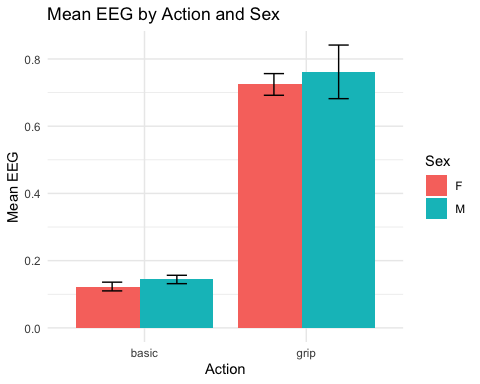
\includegraphics[keepaspectratio]{work_2_files/figure-latex/barplot-1.pdf}}

\begin{quote}
顯示不同動作(basic 與 grip)以及性別(F 與 M)在 EEG
值上的平均差異。由圖可見,在 basic 動作下,男女的 EEG 值皆偏低(約
0.1--0.15),且差異不大;然而在 grip 動作下,EEG 值明顯上升,女性約為
0.7,男性約為 0.75,整體皆高於 basic
動作。誤差線顯示數據的變異程度,男性在 grip
動作下的變異稍大於女性。整體而言,動作型態對 EEG 的影響明顯大於性別。
\end{quote}

\section{第十題:繪出``action 因子''與``sex 因子''之二階線圖(X 軸為
action
因子)}\label{ux7b2cux5341ux984cux7e6aux51faaction-ux56e0ux5b50ux8207sex-ux56e0ux5b50ux4e4bux4e8cux968eux7ddaux5716x-ux8ef8ux70ba-action-ux56e0ux5b50}

\begin{Shaded}
\begin{Highlighting}[]
\FunctionTok{ggplot}\NormalTok{(summary\_data, }\FunctionTok{aes}\NormalTok{(}\AttributeTok{x =}\NormalTok{ action, }\AttributeTok{y =}\NormalTok{ mean\_EEG, }\AttributeTok{color =}\NormalTok{ Sex, }\AttributeTok{group =}\NormalTok{ Sex)) }\SpecialCharTok{+}
  \FunctionTok{geom\_line}\NormalTok{() }\SpecialCharTok{+}
  \FunctionTok{geom\_point}\NormalTok{() }\SpecialCharTok{+}
  \FunctionTok{geom\_errorbar}\NormalTok{(}\FunctionTok{aes}\NormalTok{(}\AttributeTok{ymin =}\NormalTok{ mean\_EEG }\SpecialCharTok{{-}}\NormalTok{ se\_EEG, }\AttributeTok{ymax =}\NormalTok{ mean\_EEG }\SpecialCharTok{+}\NormalTok{ se\_EEG), }\AttributeTok{width =} \FloatTok{0.1}\NormalTok{) }\SpecialCharTok{+}
  \FunctionTok{labs}\NormalTok{(}\AttributeTok{title =} \StringTok{"Interaction Plot of EEG by Action and Sex"}\NormalTok{,}
       \AttributeTok{x =} \StringTok{"Action"}\NormalTok{,}
       \AttributeTok{y =} \StringTok{"Mean EEG"}\NormalTok{) }\SpecialCharTok{+}
  \FunctionTok{theme\_minimal}\NormalTok{()}
\end{Highlighting}
\end{Shaded}

\pandocbounded{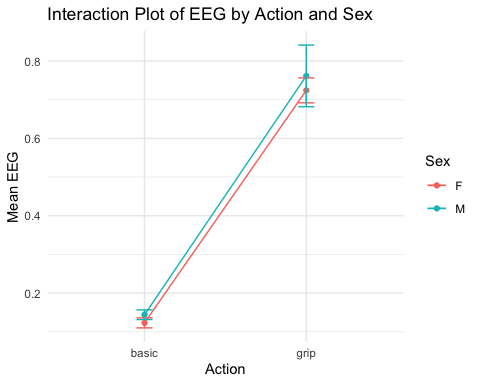
\includegraphics[keepaspectratio]{work_2_files/figure-latex/interaction-action-1.pdf}}

\begin{quote}
EEG 在不同動作(basic 與 grip)以及性別(F 與
M)下的交互作用圖。由圖可見,不論男女,EEG 值在 basic 動作下皆較低(約
0.1--0.15),在 grip 動作下明顯上升(約 0.7--0.8)。雖然男性在 grip
動作下的平均 EEG 稍高於女性,但兩者的趨勢幾乎平行,顯示性別對 EEG
的影響相對較小,而動作型態對 EEG 的影響更為顯著。誤差線則顯示,grip
動作下的變異性大於 basic 動作。
\end{quote}

\section{第十一題:繪出``action 因子''與``sex 因子''之二階線圖(X 軸為
sex
因子)}\label{ux7b2cux5341ux4e00ux984cux7e6aux51faaction-ux56e0ux5b50ux8207sex-ux56e0ux5b50ux4e4bux4e8cux968eux7ddaux5716x-ux8ef8ux70ba-sex-ux56e0ux5b50}

\begin{Shaded}
\begin{Highlighting}[]
\FunctionTok{ggplot}\NormalTok{(summary\_data, }\FunctionTok{aes}\NormalTok{(}\AttributeTok{x =}\NormalTok{ Sex, }\AttributeTok{y =}\NormalTok{ mean\_EEG, }\AttributeTok{color =}\NormalTok{ action, }\AttributeTok{group =}\NormalTok{ action)) }\SpecialCharTok{+}
  \FunctionTok{geom\_line}\NormalTok{() }\SpecialCharTok{+}
  \FunctionTok{geom\_point}\NormalTok{() }\SpecialCharTok{+}
  \FunctionTok{geom\_errorbar}\NormalTok{(}\FunctionTok{aes}\NormalTok{(}\AttributeTok{ymin =}\NormalTok{ mean\_EEG }\SpecialCharTok{{-}}\NormalTok{ se\_EEG, }\AttributeTok{ymax =}\NormalTok{ mean\_EEG }\SpecialCharTok{+}\NormalTok{ se\_EEG), }\AttributeTok{width =} \FloatTok{0.1}\NormalTok{) }\SpecialCharTok{+}
  \FunctionTok{labs}\NormalTok{(}\AttributeTok{title =} \StringTok{"Interaction Plot of EEG by Sex and Action"}\NormalTok{,}
       \AttributeTok{x =} \StringTok{"Sex"}\NormalTok{,}
       \AttributeTok{y =} \StringTok{"Mean EEG"}\NormalTok{) }\SpecialCharTok{+}
  \FunctionTok{theme\_minimal}\NormalTok{()}
\end{Highlighting}
\end{Shaded}

\pandocbounded{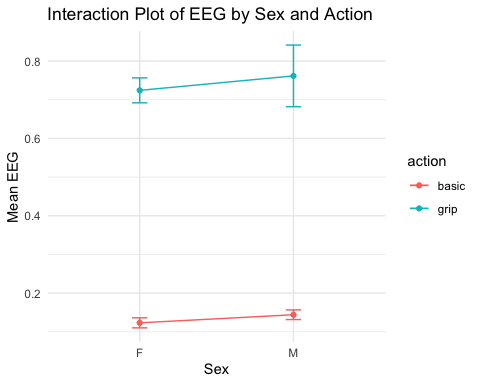
\includegraphics[keepaspectratio]{work_2_files/figure-latex/interaction-sex-1.pdf}}

\begin{quote}
顯示不同性別(F 與 M)在兩種動作(basic 與 grip)下的 EEG
平均值變化。結果顯示,不論性別,basic 動作的 EEG 值皆偏低(約
0.1--0.15),而 grip 動作的 EEG 值顯著提高(約
0.7--0.8)。在相同動作下,男性的 EEG
平均值略高於女性,但差異幅度不大。誤差線顯示 grip
動作下的數據變異性較大,basic 動作下則相對穩定。整體而言,動作型態對 EEG
的影響遠大於性別差異。
\end{quote}

\end{document}
